
Online reference books on CMake will suggest ExternalProject and FetchContent modules to deal with the management of dependencies in more complex projects. That's actually good advice, but it's often given without appropriate context. Suddenly, we're facing a lot of questions. What are these modules for? When to choose one over the other? How exactly do they work, and how do they interact with each other? Some answers are harder to find than others, and surprisingly, CMake's documentation doesn't provide a smooth introduction to the subject. Not to worry – we'll take care of it here.

\subsubsubsection{7.6.1\hspace{0.2cm}ExternalProject}

CMake 3.0.0 introduced a module called ExternalProject. As you can guess, its purpose was to add support for external projects available in online repositories. Over the years, the module was gradually extended for different needs, resulting in quite a complicated command – ExternalProject\_Add(). And I mean complicated – it accepts over 85 different options. No wonder, as it provides an impressive set of features:

\begin{itemize}
\item 
Management of directory structure for an external project

\item 
Downloading of sources from a URL (and extracting from archives if needed)

\item 
Support for Git, Subversion, Mercurial, and CVS repositories

\item 
Fetching updates if needed

\item 
Configuring and building the project with CMake, Make, or with a user-specified tool

\item 
Performing installations and running tests

\item 
Logging to files

\item 
Asking for user input from terminals

\item 
Depending on other targets

\item 
Adding custom commands/steps to the build
\end{itemize}

The ExternalProject module populates the dependencies during the build stage. For every external project added with ExternalProject\_Add(), CMake will execute the following steps:


\begin{enumerate}
\item 
mkdir – create a subdirectory for the external project

\item 
download – get the project files from a repository or URL

\item 
update – refresh the files on rerun for download methods that support delta updates

\item 
patch – optionally execute a patch command that alters downloaded files for the needs of the project

\item 
configure – execute the configure stage for CMake projects or manually specified command for non-CMake dependencies

\item 
build – perform the build stage for CMake projects, and for other dependencies, execute the make command

\item 
install – install CMake projects, and for other dependencies, execute the make install command

\item 
test – execute the dependency's tests if any of the TEST\_... options are defined
\end{enumerate}

The steps follow the preceding exact order, with the exception of the test step, which can be optionally enabled before or after the install step with the TEST\_BEFORE\_INSTALL <bool> or TEST\_AFTER\_INSTALL <bool> option.

\hspace*{\fill} \\ %插入空行
\noindent
\textbf{Downloading the step options}

We're mostly interested in options controlling the download step or how the dependency will get fetched by CMake. Firstly, we may choose to not use the CMake built-in method for that but rather provide a custom command (generator expressions are supported here):

\begin{lstlisting}[style=styleCMake]
DOWNLOAD_COMMAND <cmd>...
\end{lstlisting} 

By doing so, we tell CMake to ignore all other options for this step and just execute a system-specific command. An empty string is accepted too, and it is used to disable this step.

\hspace*{\fill} \\ %插入空行
\noindent
\textbf{Downloading dependencies from a URL}

We can provide a list of URLs to be scanned in sequence until a download succeeds. CMake will recognize whether the downloaded file is an archive and will unpack it by default:

\begin{lstlisting}[style=styleCMake]
URL <url1> [<url2>...]
\end{lstlisting} 

Additional options allow us to customize the behavior of this method further:

\begin{itemize}
\item 
URL\_HASH <algo>=<hashValue> – checks whether a downloaded file's checksum generated by <algo> matches the provided <hashValue>. It is recommended to guarantee the integrity of downloads. The MD5, SHA1, SHA224, SHA256, SHA384, SHA512, SHA3\_224, SHA3\_256, SHA3\_384, and SHA3\_512 supported algorithms are defined by the string(<HASH>) command. For MD5, we can use a shorthand option, URL\_MD5 <md5>.

\item 
DOWNLOAD\_NO\_EXTRACT <bool> – explicitly disables extraction after downloading. We may consume the filename of downloaded files in the follow-up steps by accessing the <DOWNLOADED\_FILE> variable.

\item 
DOWNLOAD\_NO\_PROGRESS <bool> – don't log download progress.

\item 
TIMEOUT <seconds> and INACTIVITY\_TIMEOUT <seconds> – timeouts to terminate the download after a fixed total time or period of inactivity.

\item 
HTTP\_USERNAME <username> and HTTP\_PASSWORD <password> – options to provide values for HTTP authentication. Always be sure to avoid hardcoding any credentials in your projects.

\item 
HTTP\_HEADER <header1> [<header2>…] – sends additional headers with your HTTP request. Use this to access content in AWS or pass some custom tokens.

\item 
TLS\_VERIFY <bool> – verifies the SSL certificate. If this is not set, CMake will read this setting from the CMAKE\_TLS\_VERIFY variable, which is set to false by default. Skipping TLS verification is an unsafe, bad practice and should be avoided, especially in production environments.

\item 
TLS\_CAINFO <file> – this is useful if your company is issuing self-signed SSL certificates. This option provides a path to the authority file; if it isn't specified, CMake will read this setting from the CMAKE\_TLS\_CAINFO variable.
\end{itemize}

\hspace*{\fill} \\ %插入空行
\noindent
\textbf{Downloading dependencies from Git}

To download dependencies from Git, you'll need to make sure that the host has Git 1.6.5 or later installed. The following options are required to clone from Git:

\begin{lstlisting}[style=styleCMake]
GIT_REPOSITORY <url>
GIT_TAG <tag>
\end{lstlisting} 

Both <url> and <tag> should be in formats understood by the git command. Additionally, it is recommended to use a specific git hash to make sure that produced binaries can be traced to a specific commit and no unnecessary git fetch executions are made. If you insist on using a branch, use remote names such as origin/main. This guarantees the correct synchronization of the local clone.

Additional options are as follows:

\begin{itemize}
\item 
GIT\_REMOTE\_NAME <name> – the remote name, which defaults to origin.

\item 
GIT\_SUBMODULES <module>... – specifies which submodules should be updated. Since 3.16, this value defaults to none (previously, all submodules were updated).

\item 
GIT\_SUBMODULES\_RECURSE 1 – enables the recursive update of submodules.

\item 
GIT\_SHALLOW 1 – performs a shallow clone (don't download historical commits). This option is recommended for performance.

\item 
TLS\_VERIFY <bool> – this option was explained in the Downloading dependencies from a URL section. It is also available for Git, and should be enabled for security.
\end{itemize}

\hspace*{\fill} \\ %插入空行
\noindent
\textbf{Downloading dependencies from Subversion}

To download from Subversion, we should specify the following options:

\begin{lstlisting}[style=styleCMake]
SVN_REPOSITORY <url>
SVN_REVISION -r<rev>
\end{lstlisting} 

Additionally, we may provide the following:

\begin{itemize}
\item 
SVN\_USERNAME <user> and SVN\_PASSWORD <password> – credentials for checkout and update. As always, avoid hardcoding them in your projects.
	
\item 
SVN\_TRUST\_CERT <bool> – skips the verification of the Subversion server site certificate. Only use this option if the network path to the server and its integrity are trustworthy. It is disabled by default.
\end{itemize}

\hspace*{\fill} \\ %插入空行
\noindent
\textbf{Downloading dependencies from Mercurial}

This mode is very straightforward. We need to provide two options and we're done:

\begin{lstlisting}[style=styleCMake]
HG_REPOSITORY <url>
HG_TAG <tag>
\end{lstlisting} 

\hspace*{\fill} \\ %插入空行
\noindent
\textbf{Downloading dependencies from CVS}

To check out modules from CVS, we need to provide these three options:

\begin{lstlisting}[style=styleCMake]
CVS_REPOSITORY <cvsroot>
CVS_MODULE <module>
CVS_TAG <tag>
\end{lstlisting} 

\hspace*{\fill} \\ %插入空行
\noindent
\textbf{Update step options}

By default, the update step will re-download the external project's files if the download method supports updates. We can override this behavior in two ways:

\begin{itemize}
\item 
Provide a custom command to be executed during the update with UPDATE\_COMMAND <cmd>.

\item 
Completely disable the update step (to allow building with a disconnected network) – UPDATE\_DISCONNECTED <bool>. Do note that the download step (during the first build) will still happen.
\end{itemize}

\hspace*{\fill} \\ %插入空行
\noindent
\textbf{Patch step options}

Patch is an optional step that will execute after the source is fetched. To enable it, we need to specify the exact command we want to execute with:

\begin{lstlisting}[style=styleCMake]
PATCH_COMMAND <cmd>...
\end{lstlisting} 

CMake documentation warns that some patches may be more "sticky" than others. For example, in Git, changed files don't get restored to the original state during the update, and we need to be careful to avoid incorrectly patching the file twice. Ideally, the patch command should be really robust and idempotent.

\begin{tcolorbox}[colback=blue!5!white,colframe=blue!75!black,title=Important Note]
The previously mentioned lists of options contain only the most useful entries. Be sure to reference the official documentation for more details and a description of options for other steps: \url{https://cmake.org/cmake/ help/latest/module/ExternalProject.html}.
\end{tcolorbox}

\hspace*{\fill} \\ %插入空行
\noindent
\textbf{Using ExternalProject in practice}

The fact that dependency is populated at the build stage is very important, and it has two effects – the namespaces of projects are completely separate, and targets defined by any external project are not visible in the main project. The latter is especially painful, as we can't use target\_link\_libraries() in the same fashion as we would after using the find\_package() command. This is because of a disjoint of two configuration stages. The main project has to finish the configuration stage and start the build stage before the dependency is downloaded and configured. This is an issue, but we'll learn how to deal with that in a second. For now, let's see how ExternalProject\_Add() would work with the yaml-cpp library that we used in the previous examples:

\begin{lstlisting}[style=styleCMake]
# chapter07/08-external-project-git/CMakeLists.txt

cmake_minimum_required(VERSION 3.20.0)
project(ExternalProjectGit CXX)

add_executable(welcome main.cpp)
configure_file(config.yaml config.yaml COPYONLY)

include(ExternalProject)
ExternalProject_Add(external-yaml-cpp
	GIT_REPOSITORY https://github.com/jbeder/yaml-cpp.git
	GIT_TAG yaml-cpp-0.6.3
)
target_link_libraries(welcome PRIVATE yaml-cpp)
\end{lstlisting} 

These are the steps taken to build this project:

\begin{itemize}
\item 
We included the ExternalProject module to access its functions.

\item 
We called the FindExternalProject\_Add() command, which tasks the build stage with downloading the necessary files, and configuring, building, and installing the dependency in our system.
\end{itemize}

We need to be cautious here and understand that this example only works because the yaml-cpp library has an installation stage defined in its CMakeLists.txt. This stage copies the library files to the standard locations in the system. The yaml-cpp argument to the target\_link\_libraries() command is interpreted by CMake as a direct argument to the linker – -lyaml-cpp. This behavior differs from the previous examples, where we explicitly defined the yaml-cpp target. If the library wouldn't provide an installation stage (or the name of the binary version wouldn't match), the linker would throw an error.

At this point, we should dive deeper into the configuration of each stage and explain how to use different download methods. We'll get to that in the FetchContent section, but first, let's get back to the problem of late dependency fetching by ExternalProject. We cannot use targets of external projects in the compilation stage because that stage has already finished by the time these projects are being fetched. CMake will explicitly protect the target created with FindExternalProject\_Add() by marking it with a special UTILITY type. When you mistakenly try to use such a target in the main project (perhaps to link it), CMake will throw an error:

\begin{tcblisting}{commandshell={}}
Target "external-yaml-cpp-build" of type UTILITY may not be
linked into another target.
\end{tcblisting}

To get around this limitation, we can technically create another target, an IMPORTED library, and use that instead (just as we did earlier in this chapter with FindPQXX.cmake). But this is an awful lot of work. What's worse is that CMake actually understands the targets created by the external CMake projects (since it builds them). Repeating those declarations in the main project wouldn't be a very DRY practice.

Another possible solution is to extract whole dependency fetching and building to a separate sub-project and build that during the configuration stage. To make it happen, we'd need to start another instance of CMake with execute\_process(). With some trickery and the add\_subdirectory() command, we can then consume this sub-project's list files and binaries into the main project. This approach (sometimes called the super-build) is outdated and unnecessarily complex. I won't go into the details here, as it wouldn't be very useful for beginners. If you're curious, read this great article by Craig Scott: \url{https://crascit.com/2015/07/25/cmake-gtest/}.

To sum it up, ExternalProject can get us out of a bind when there are namespacing collisions across projects, but in all other cases, FetchContent is far superior. Let's figure out why

\subsubsubsection{7.6.2\hspace{0.2cm}FetchContent}

Nowadays, it is recommended to go with the FetchContent module to import external projects. This module has been available in CMake since version 3.11, but we recommend using at least 3.14 to work with it effectively.

Essentially, it's a high-level wrapper around ExternalProject, offering similar functionality and more. The key difference is in the stage of execution – unlike ExternalProject, FetchContent populates dependencies during the configuration stage, bringing all the targets declared by an external project to the scope of the main project. This way, we can use them exactly like the ones we defined ourselves.

The usage of FetchContent module requires three steps:

\begin{enumerate}
\item 
Include the module in your project with include(FetchModule).

\item 
Configure dependencies with the FetchContent\_Declare() command.

\item 
Populate dependencies with the FetchContent\_MakeAvailable() command – download, build, install, and add its list files to the main project and parse.
\end{enumerate}

You may ask yourself why the Declare and MakeAvailable commands were separated. This was done to enable configuration overrides in hierarchical projects. Here's a scenario – a parent project depends on the A and B external libraries. The A library also depends on B, but authors of the A library are still using an old version, different from the parent project (Figure 7.1):

\begin{center}
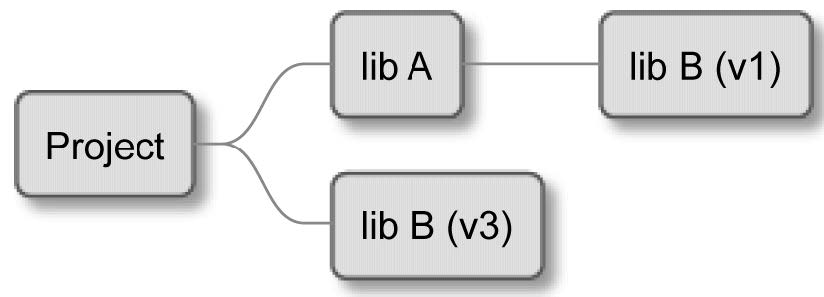
\includegraphics[width=0.5\textwidth]{content/2/chapter7/images/1.jpg}\\
Figure 7.1 – The hierarchical project
\end{center}

What's more, the dependency on the B library is optional, depending on the configuration (let's say it's OS-specific). MakeAvailable can't both configure and populate the dependency because to override the version in the A library, the parent project would be forced to populate the dependency regardless of its final necessity in the A library.

By virtue of having a separate configuration step, we're able to specify a single version in the parent project and have it used in all sub-projects and dependencies:

\begin{lstlisting}[style=styleCMake]
FetchContent_Declare(
	googletest
	GIT_REPOSITORY https://github.com/google/googletest.git
	# release-1.11.0
	GIT_TAG e2239ee6043f73722e7aa812a459f54a28552929
)
\end{lstlisting} 

Any subsequent calls to FetchContent\_Declare() with googletest as the first argument will be ignored to allow the project highest in the hierarchy to decide how to handle this dependency.

The signature of the FetchContent\_Declare() command is exactly the same as ExternalProject\_Add():

\begin{lstlisting}[style=styleCMake]
FetchContent_Declare(<depName> <contentOptions>...)
\end{lstlisting} 

This is no coincidence – these arguments will be stored by CMake until the FetchContent\_MakeAvailable() is called and population is necessary. Then, they will be forwarded internally to the ExternalProject\_Add() command. However, not all of the options are allowed. We can specify any options of the download, update, or patch steps but not the configure, build, install, or test steps.

When the configuration is ready, we'll populate the dependencies like so:

\begin{lstlisting}[style=styleCMake]
FetchContent_MakeAvailable(<depName>)
\end{lstlisting} 

This will download the files and read the targets into the project, but what actually happens during this call? FetchContent\_MakeAvailable() was added to CMake 3.14 to wrap the most commonly used scenario in a single command. In Figure 7.2, you can see the details of this process:

\begin{enumerate}
\item 
Call FetchContent\_GetProperties() to read the configuration set by FetchContent\_Declare() from the global variables to local variables.

\item 
Check (case-insensitively) whether the dependency with this name was already populated to avoid downloading it twice. If so, stop here.

\item 
Call FetchContent\_Populate(). It will configure the wrapped ExternalProject module by forwarding options we have set (but skipping the disabled ones) and downloading the dependency. It will also set some variables to prevent re-downloading on subsequent calls and forward the necessary paths to the next command.

\item 
Finally, add\_subdirectory() is called with source and build trees as arguments to tell the parent project where the list files are and where to put the build artifacts.
\end{enumerate}

By calling add\_subdirectory(), CMake effectively performs the configuration stage of the fetched project and retrieves any targets defined there in the current scope. How convenient!

\begin{center}
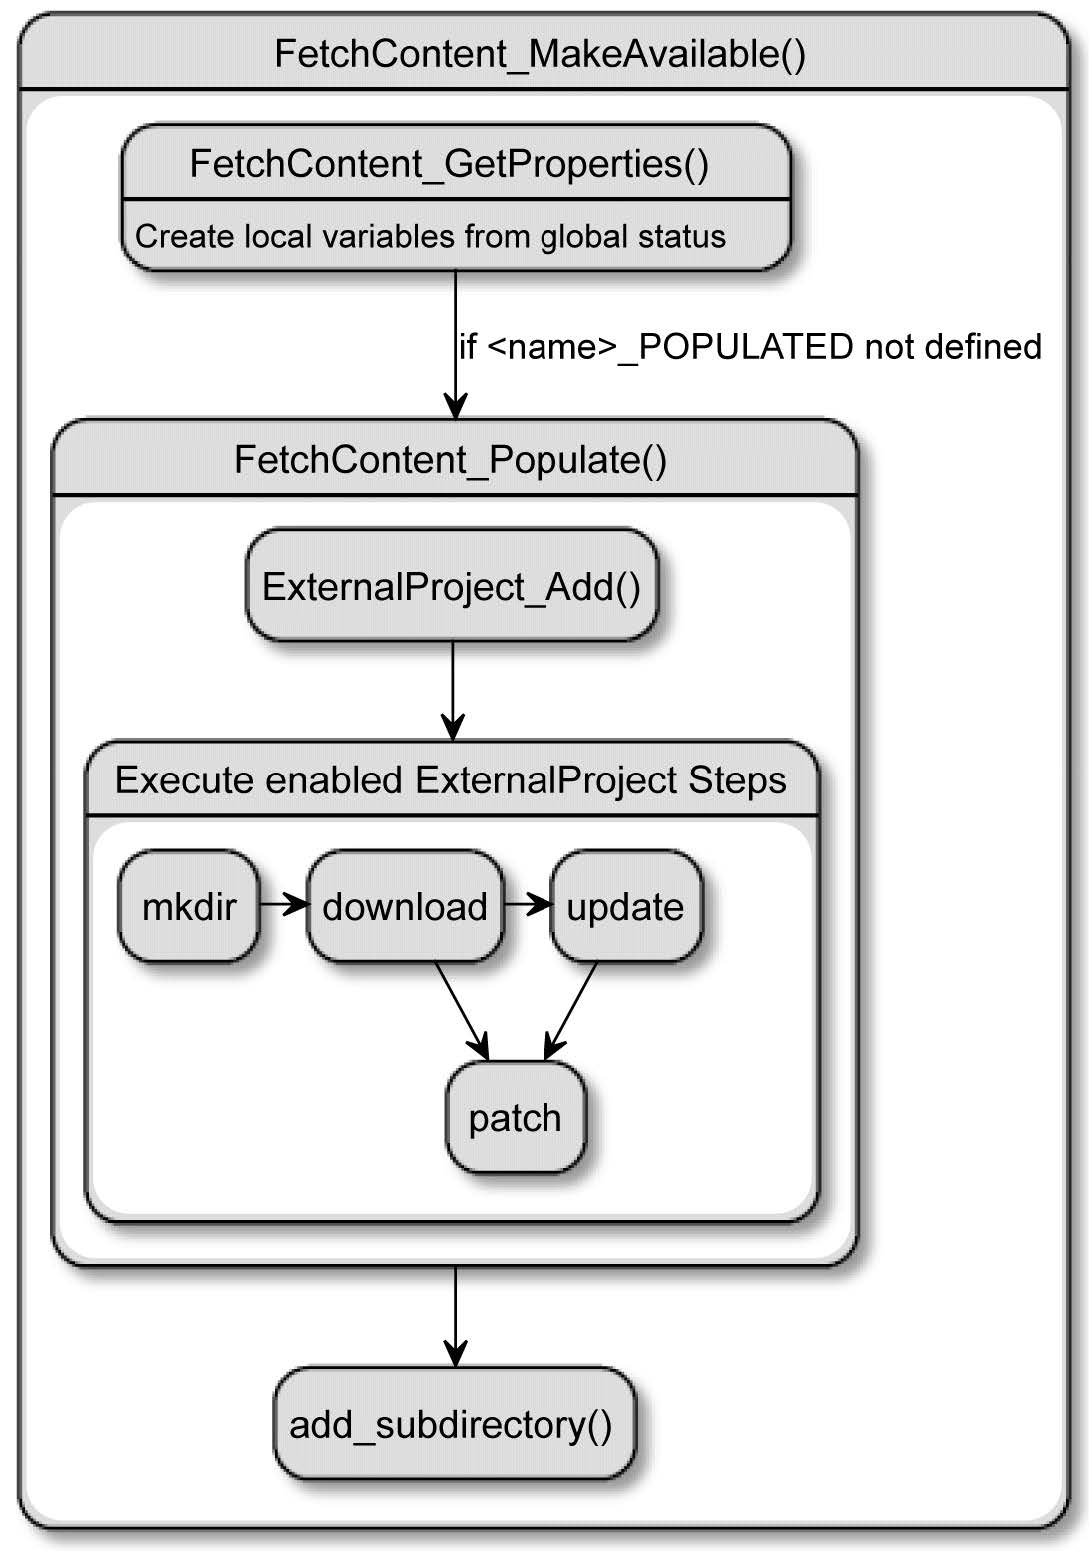
\includegraphics[width=0.8\textwidth]{content/2/chapter7/images/2.jpg}\\
Figure 7.2 – How FetchContent\_MakeAvailable() wraps calls to ExternalProject
\end{center}

Obviously, we may have a situation where two unrelated projects declare a target with the same name. This is a problem that can only be solved by falling back to ExternalProject or other methods. Luckily, it doesn't happen too often.

For this explanation to be complete, it has to be complemented with a practical example. Let's see how the list file from the previous section changes when we switch to FetchContent:

\begin{lstlisting}[style=styleCMake]
# chapter07/09-fetch-content/CMakeLists.txt

cmake_minimum_required(VERSION 3.20.0)
project(ExternalProjectGit CXX)

add_executable(welcome main.cpp)
configure_file(config.yaml config.yaml COPYONLY)

include(FetchContent)
FetchContent_Declare(external-yaml-cpp
	GIT_REPOSITORY https://github.com/jbeder/yaml-cpp.git
	GIT_TAG yaml-cpp-0.6.3
)
FetchContent_MakeAvailable(external-yaml-cpp)
target_link_libraries(welcome PRIVATE yaml-cpp)
\end{lstlisting} 

ExternalProject\_Add was directly replaced with FetchContent\_Declare, and we added another command – FetchContent\_MakeAvailable. The changes in code are minuscule, but the practical differences are huge! We can explicitly access the targets created by the yaml-cpp library. To prove it, we'll use a CMakePrintHelpers helper module and add these lines to the previous file:

\begin{lstlisting}[style=styleCMake]
include(CMakePrintHelpers)
cmake_print_properties(TARGETS yaml-cpp
	PROPERTIES TYPE SOURCE_DIR)
\end{lstlisting} 

Now, the configuration stage will print the following output:

\begin{lstlisting}[style=styleCMake]
Properties for TARGET yaml-cpp:
	yaml-cpp.TYPE = "STATIC_LIBRARY"
	yaml-cpp.SOURCE_DIR = "/tmp/b/_deps/external-yaml-cpp-src"
\end{lstlisting} 

The target exists; it's a static library, and its source directory resides inside the build tree. Using the same helper to debug the target in the ExternalProject example simply returns:

\begin{tcblisting}{commandshell={}}
No such TARGET "yaml-cpp" !
\end{tcblisting}

The target isn't recognized during the configuration stage. This is why FetchContent is much better and should be used wherever possible.




